% HMC Math dept HW template example
% v0.04 by Eric J. Malm, 10 Mar 2005
\documentclass[10pt,a4paper,boxed]{hmcpset}

% set 1-inch margins in the document
% \usepackage[margin=1in]{geometry}
\usepackage{enumerate}
\usepackage{todonotes}
%\usepackage{tikz}
%\usetikzlibrary{positioning}
\usepackage{subfig} % subfigures in figures.	
\usepackage{pgfplots}
\usepackage{amsmath}
\usepackage{amsfonts}
\usepackage{amssymb}

%% work around for subfig and asy environment
\makeatletter
\newsavebox{\sfe@box}
\newenvironment{subfloatenv}[2]{%
\def\sfe@caption{#1}%
\def\sfe@label{#2}%
\setbox\sfe@box\hbox\bgroup\color@setgroup}%
{\color@endgroup\egroup\subfloat[\sfe@caption]%
{\usebox{\sfe@box}\label{\sfe@label}}}
\makeatother

% include this if you want to import graphics files with /includegraphics
\usepackage{graphicx}

\renewcommand*{\familydefault}{\sfdefault}
\newcommand{\vect}[1]{\mathbf{#1}}

\def\correct{\tikz\fill[scale=0.4,color=green](0,.35) -- (.25,0) -- (1,.7) -- (.25,.15) -- cycle; }

\def\examrelevant{\color{red}Exam relevant!}


\usepackage{ amssymb }

%\tikzset{node distance=2cm, inner/.style={draw,circle}, leaf/.style={draw,rectangle}}

\usepackage{hyperref}

% info for header block in upper right hand corner
\name{Lukas Gesing, Patrick Kaster}
\class{MA-INF 4201 - Artificial Life}
\assignment{Exercise Sheet 3}
% \duedate{09/03/2004}

\begin{document}
\begin{problem}[Assignment 16] \correct
\end{problem}
\begin{solution}
The rule has a silent state, if a dead cell is has no neighbours. I wouldn't characterize it as totalistic, without having specified some kind of binary value to the neighbouring cells. It is symmetric though, since the 23/3 rule doesn't depend on the position of the neighbours. So each symmetric configuration will lead to the same result. It is legal, since it is symmetric and shows a silent state. It is not peripheral, since the outcome is in any case dependent on whether the cell os dead or alive.\\

\underline{In shot:} 
    \begin{itemize} 
        \item silent state \checkmark
        \item totalistic $\times$
        \item symmetric \checkmark
        \item peripheral $\times$
        \item legal \checkmark
    \end{itemize}

\end{solution}


\begin{problem}[Assignment 17] \correct
\end{problem}
\begin{solution}
That it is possibly to create a Game of Life pattern that can grow infinitely.
\end{solution}


\begin{problem}[Assignment 18] \correct
\end{problem}
\begin{solution}
Class IV. It's evolution leads to complex structures, even releasing a glider at some point of it's evolution, and the \emph{r-pentomino} is long lived.
\end{solution}


\begin{problem}[Assignment 19] \examrelevant
\end{problem}
\begin{solution}
\marginpar[left text]{Was asked in each exam in the past!!! Just lern the pattern by heart.}

\begin{figure}[h]
\centering
    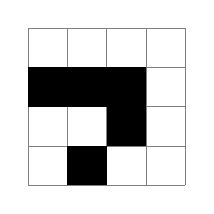
\begin{tikzpicture}
        \draw[step=0.5cm,gray,very thin] (0,0) grid (2,2);
        \fill[black] (0.5,0) rectangle (1,0.5);
        \fill[black] (1,0.5) rectangle (1.5,1);
        \fill[black] (0,1) rectangle (1.5,1.5);
    \end{tikzpicture}
    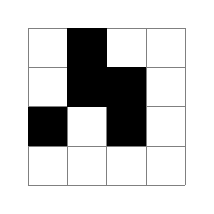
\begin{tikzpicture}
        \draw[step=0.5cm,gray,very thin] (0,0) grid (2,2);
        \fill[black] (0,0.5) rectangle (0.5,1);
        \fill[black] (1,0.5) rectangle (1.5,1);
        \fill[black] (0.5,1) rectangle (1.5,1.5);
        \fill[black] (0.5,1.5) rectangle (1,2);
    \end{tikzpicture}
    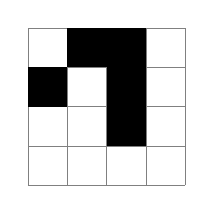
\begin{tikzpicture}
        \draw[step=0.5cm,gray,very thin] (0,0) grid (2,2);
        \fill[black] (0,1) rectangle (0.5,1.5);
        \fill[black] (0.5,1.5) rectangle (1.5,2);
        \fill[black] (1,0.5) rectangle (1.5,1.5);
    \end{tikzpicture}
    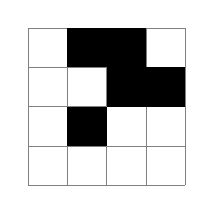
\begin{tikzpicture}
        \draw[step=0.5cm,gray,very thin] (0,0) grid (2,2);
        \fill[black] (0.5,0.5) rectangle (1,1);
        \fill[black] (0.5,1.5) rectangle (1.5,2);
        \fill[black] (1,1) rectangle (2,1.5);
    \end{tikzpicture}
        \caption{Possible solution}
\end{figure}  
\end{solution}

\newpage

\begin{problem}[Assignment 20]
\end{problem}
\begin{solution}
A cellular d-graph automaton $\mathcal{M}$ is a triple ($\Gamma$, $M$, $H$), where
    \begin{itemize} 
        \item[$\Gamma$] is a d-graph, ($N$, $A$, $f$, $g$) on the label set $L$
        \item[$M$] is a finite-state automaton ($Q$, $\delta$), where \\
                    $Q$ is a finite nonempty set of states such that $L \subseteq Q$\\
                    $\delta$ is a transition function from $Q \times Z^d_d \times Q^d$ into subsets of $Q$ which maps any triple whose first term is \# into {\#}
        \item[$H$] is a mapping from $N$ into $Z^d_d$; the image $H(n)=(t_1.....t_d) \in Z^d_d$ called the neighbor vector of $n$
    \end{itemize}
If the range of $\delta$ is the singleton subsets of $Q$, then it is called a deter- ministic cellular d-graph automaton and $\delta$ may be considered as a function from $Q × Z^d_d × Z^d_d$ into $Q$.\footnote{http://www.sciencedirect.com/science/article/pii/S0019995879902882}
\end{solution}


\begin{problem}[Assignment 22]
\end{problem}
\begin{solution}

\centering
   \begin{itemize}
     \item[] overcroweding $\rightarrow$ at least 4
     \item[] not birth $\rightarrow$ 4 cells or more
   \end{itemize}
   
\begin{figure}[h]
\centering
    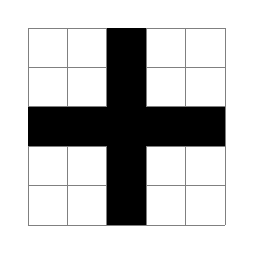
\begin{tikzpicture}
        \draw[step=0.5cm,gray,very thin] (0,0) grid (2.5,2.5);
        \fill[black] (1,0) rectangle (1.5,2.5);
        \fill[black] (0,1) rectangle (2.5,1.5);
    \end{tikzpicture}
    \caption{Possible solution}
\end{figure}  

\end{solution}


\begin{problem}[Assignment 23]
\end{problem}
\begin{solution}

\end{solution}

\end{document}

